%!TEX program = xelatex
\documentclass{standalone}
\usepackage{tikz}
\usetikzlibrary{arrows}
\usepackage{fontspec}
    \setmainfont{Charis SIL}
\begin{document}
% In the preamble:

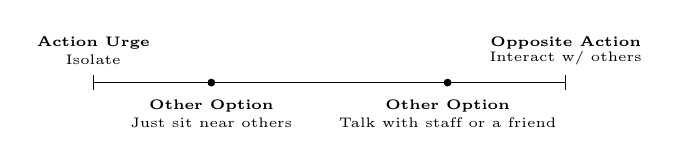
\begin{tikzpicture}[label distance=5mm]
  \draw [|-, solid] (-3,0) node [] {} -- (-0.45,0) node[midway,above,sloped] (TextNode) {\tiny };
  \draw [-, solid] (-0.45,0) node [] {} -- (0.45,0) node[midway,above,sloped] (TextNode) {\tiny };
  \draw [-|, solid] (0.45,0) node [] {} -- (3,0) node[midway,above,sloped] (TextNode) {\tiny };

      \draw (-1.5,-0) node[circle,fill,inner sep=1pt]{};
      \draw (1.5,-0) node[circle,fill,inner sep=1pt]{};

 \draw (-1.5,-0.5) node[align=center, anchor=south]{\tiny \textbf{Other Option}};
  \draw (-1.5,-0.7) node[align=center, anchor=south]{\tiny Just sit near others};
   \draw (1.5,-0.5) node[align=center, anchor=south]{\tiny \textbf{Other Option}};
  \draw (1.5,-0.7) node[align=center, anchor=south]{\tiny Talk with staff or a friend};

 \draw (-3,0.3) node[align=center, anchor=south]{\tiny \textbf{Action Urge}};
  \draw (-3,0.1) node[align=center, anchor=south]{\tiny Isolate};
 \draw (3,0.3) node[align=center, anchor=south]{\tiny \textbf{Opposite Action}};
  \draw (3,0.1) node[align=center, anchor=south]{\tiny Interact w/ others};

\end{tikzpicture}

\end{document}
